\documentclass{article} %article类型的文档只能有英文,编译器为pdfLaTeX

\usepackage{amsmath} %数学公式
\usepackage{graphicx} %图片加载
\usepackage{float} 
\usepackage{subcaption} %插入子图
\usepackage{fancyhdr} %页眉页脚设置

\usepackage{enumerate} %项目符号
\usepackage{lastpage} %总页数


\usepackage{caption} 
\usepackage{cite} %引用
\usepackage{times} %设定为Times New Roman字体
\usepackage{hyperref} %超链接
\usepackage{booktabs} %line type

\usepackage{geometry} %此宏包帮助设置页面宽度
\geometry{a4paper,scale=0.8} %设置A4页面,填充80%

\usepackage{threeparttable} %三线表,论文规范表格
\usepackage{pbox} % set maximum length for a table
\usepackage{multirow} %表格多行
\usepackage{makecell} %帮助表格内换行
\usepackage{footnote} %脚注

\usepackage{listings} %插入代码
\bibliographystyle{plain} %设置参考文献,括号内可有不同风格
\newcommand{\upcite}[1]{\textsuperscript{\textsuperscript{\cite{#1}}}} %设置上标引用



\newcommand{\cev}[1]{\reflectbox{\ensuremath{\vec{\reflectbox{\ensuremath{#1}}}}}}

 %类似头文件的存在,也可以直接把代码放到这里
\title{A simple $\LaTeX$ template}
\author{Your name.}
\date{} %设置日期,默认当天

\begin{document}
\begin{figure}
    \centering %居中
    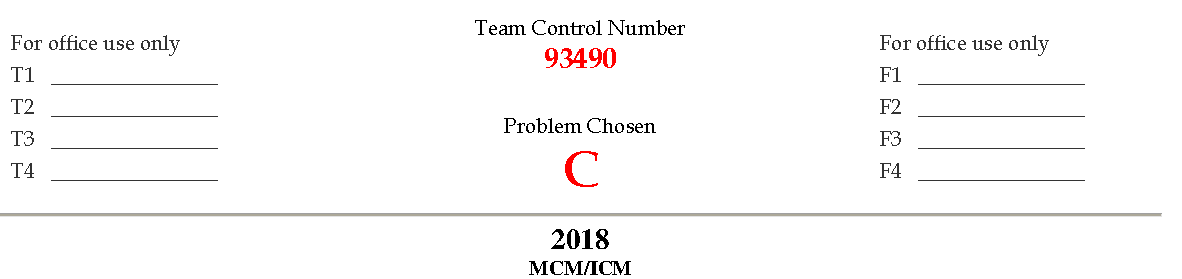
\includegraphics[width=\linewidth]{fig/sheethead.pdf} %插入图片,设置宽度为0.5倍行宽
\end{figure}
\maketitle %制作好标题

\section{Section 1}
\subsection{Subsection 1 of Section 1}
Mater Eagle Fly High is shown in figure \ref{fig:my_label}.%ref用于引用标签,特别是会随着图片的标签更新而更新

\section{Insert a figure}
%下面插入一张图片
\begin{figure}[H] %后面的[]里面可以设置图片的位置,自行百度
    \centering %居中
    
\includegraphics[width=0.5\linewidth]{fig/fly.jpg} %插入图片,设置宽度为0.5倍行宽
    \caption{Mater Eagle Fly High}
    \label{fig:my_label} %设置图片标签,方便引用
\end{figure}

\section{Insert an equation}
%下面插入一个公式(会自带编号)
\begin{equation}
    E=m c^2
\end{equation}

\section{Insert mathematical signs in texts}
%下面在正文中插入数学符号
You can also insert mathematical signs in your texts, like this: $E=m c^2$ is found by Einstein. 

\section{Insert a threeparttable} 
%下面插入一个三线表
\begin{table}[H]
\centering
    \begin{threeparttable}
        \begin{tabular}{ll}
        \toprule
        Name         & Student ID \\
        \midrule
        Ga Zhang     & 2014010330 \\
        Chuankai Liu & 2016010324 \\
        Haoxin Deng  & 2016010278 \\
        \bottomrule
        \end{tabular}
    \end{threeparttable}
\end{table}

\section{Insert list of items}
%逐条插入
Members of the team 'real fans' include:
\begin{itemize} %无编号分点

    \item Ga Zhang
    \item Chuankai Liu
    \item Haoxin Deng
\end{itemize}

To put an elephant to a refrigerator, you just need to follow these tips:
\begin{enumerate} %有编号分点
    \item Open the refrigerator.
    \item Let the elephant in.
    \item Close the refrigerator.
\end{enumerate}

\section{Insert citation}
%引用参考文献
We must follow Deng Xiaoping's theory.\upcite{jiang1997hold} %括号中相当于参考文献的“变量名”,见ref.bib文件


%下面加入参考文献,文献来自ref.bib文件
\bibliography{ref}
\end{document}
